\chapter{Literature Review}
The problem of proving a tight bound on the stretch factor of the Delaunay triangulation has received considerable attention in the area of computational geometry. And there is a long list of results on improving both the lower and upper bounds.

% \textcolor{blue}{(Maybe add a graph as a timeline for both lower bound & upper bound, but in what form (arrows, direction, ...)? Or, too many figures?)}

\section{On the Lower Bound}

\subsection{\texorpdfstring{$\pi/2\approx 1.5708$}     {Lg}, Chew in 1989}

As we mentioned in section 1.2, the property stretch factor of Delaunay triangulation was first introduced by Chew\cite{chew} in 1987. Although the main result was on TD (triangle distance) Delaunay triangulation, Chew discussed the stretch factor in the case of standard Delaunay triangulation at the end of the paper. Chew pointed out it was clear that $\pi/2$ is a lower bound by constructing a set of points on a unit circle. 

Bose et al.\cite{BoseCGTA} wrote a rigor proof based on Chew's idea and gave a detailed illustration as Figure~\ref{fig:pi:2}. We first distribute a set of points uniformly on a unit circle. Choose two points $p$ and $p'$ that are diametrically opposite with each other. Then, let us construct a triangulation with all edges which are nearly perpendicular to $\overline{pp'}$. Since all points are on the same circle, the triangulation must be a Delaunay triangulation. Also, for every pair of points, the shortest path should be the one along the boundary of the circle. Therefore, as the set of points become larger, the ratio for the pair of $p$ and $p'$ approaches $\pi/2$, and that ratio is always the maximum among all pairs. Thus, the stretch factor would be close to $\pi/2$.

\begin{figure}[ht]
\centering
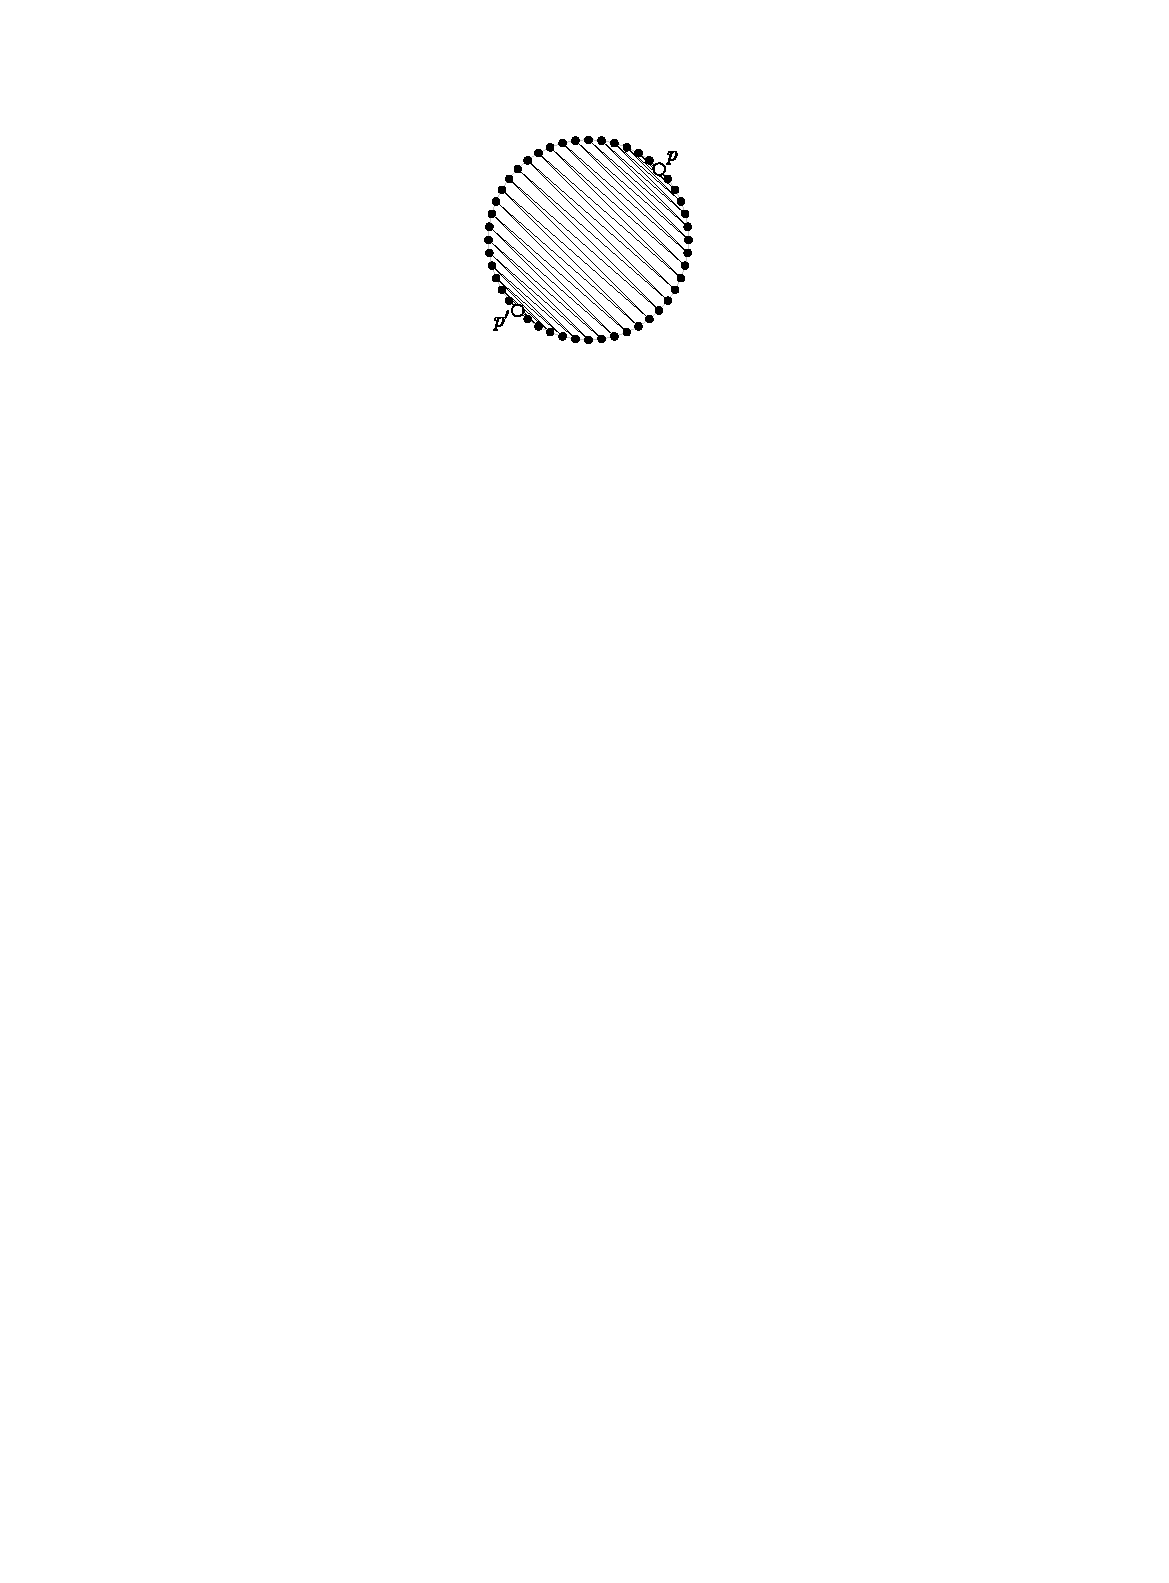
\includegraphics[width=50mm]{Figures/pi:2.pdf}
% \decoRule
\caption[An instance that the stretch factor approaches $\pi/2$]{An instance that the stretch factor approaches $\pi/2$. Reprinted from Bose et al.\cite{BoseCGTA}.} 
\label{fig:pi:2}
\end{figure}









\subsection{\texorpdfstring{$1.5846$}{Lg}, Bose et al. in 2009}
It has long been conjectured that the lower bound of stretch factor can be at most $\pi/2$ until Bose et al. \cite{BoseCGTA} constructed a point set with the  stretch factor great than 1.5846 in 2009.
Their construction is based on the following  observation. Consider a sector of a unit circle as in Figure~\ref{fig:Bose_a}. According to the figure, there are two types of locally optimal path from $p$ to $q$: 1)the arc $pq$  around the sector, and 2) the path consisting of the arc $pq'$ followed by the segment $q'q$. Bose et al. proved that when $\beta$ under a certain condition relative to $\theta$,  path 1 is shorter than path 2. Thus, if we can make every $\beta$ meet the appropriate condition, the observation would guarantee the path along the perimeter as the shortest. The paper provided a model made up two unit semicircles with a gap $d$. Figure~\ref{fig:Bose_c} is a construction with a stretch factor of $1.5810$. 

Bose et al. stated that  the instance in Figure~\ref{fig:Bose_c} is valid for a set of points in convex position, which is a more general definition comparing with that in plane. Also,  they claimed they could increase the stretch factor slightly by replacing the two straight segments with points on a common circle $C$ and adding four shield points $s$. (Figure~\ref{fig:Bose_d}) Then, no edges inside the polygon is used. And the lower bound of stretch factor for points in the plane was improved to be $1.5846$.



\begin{figure}[ht]
        \centering
        \begin{subfigure}[b]{0.475\textwidth}
            \centering
            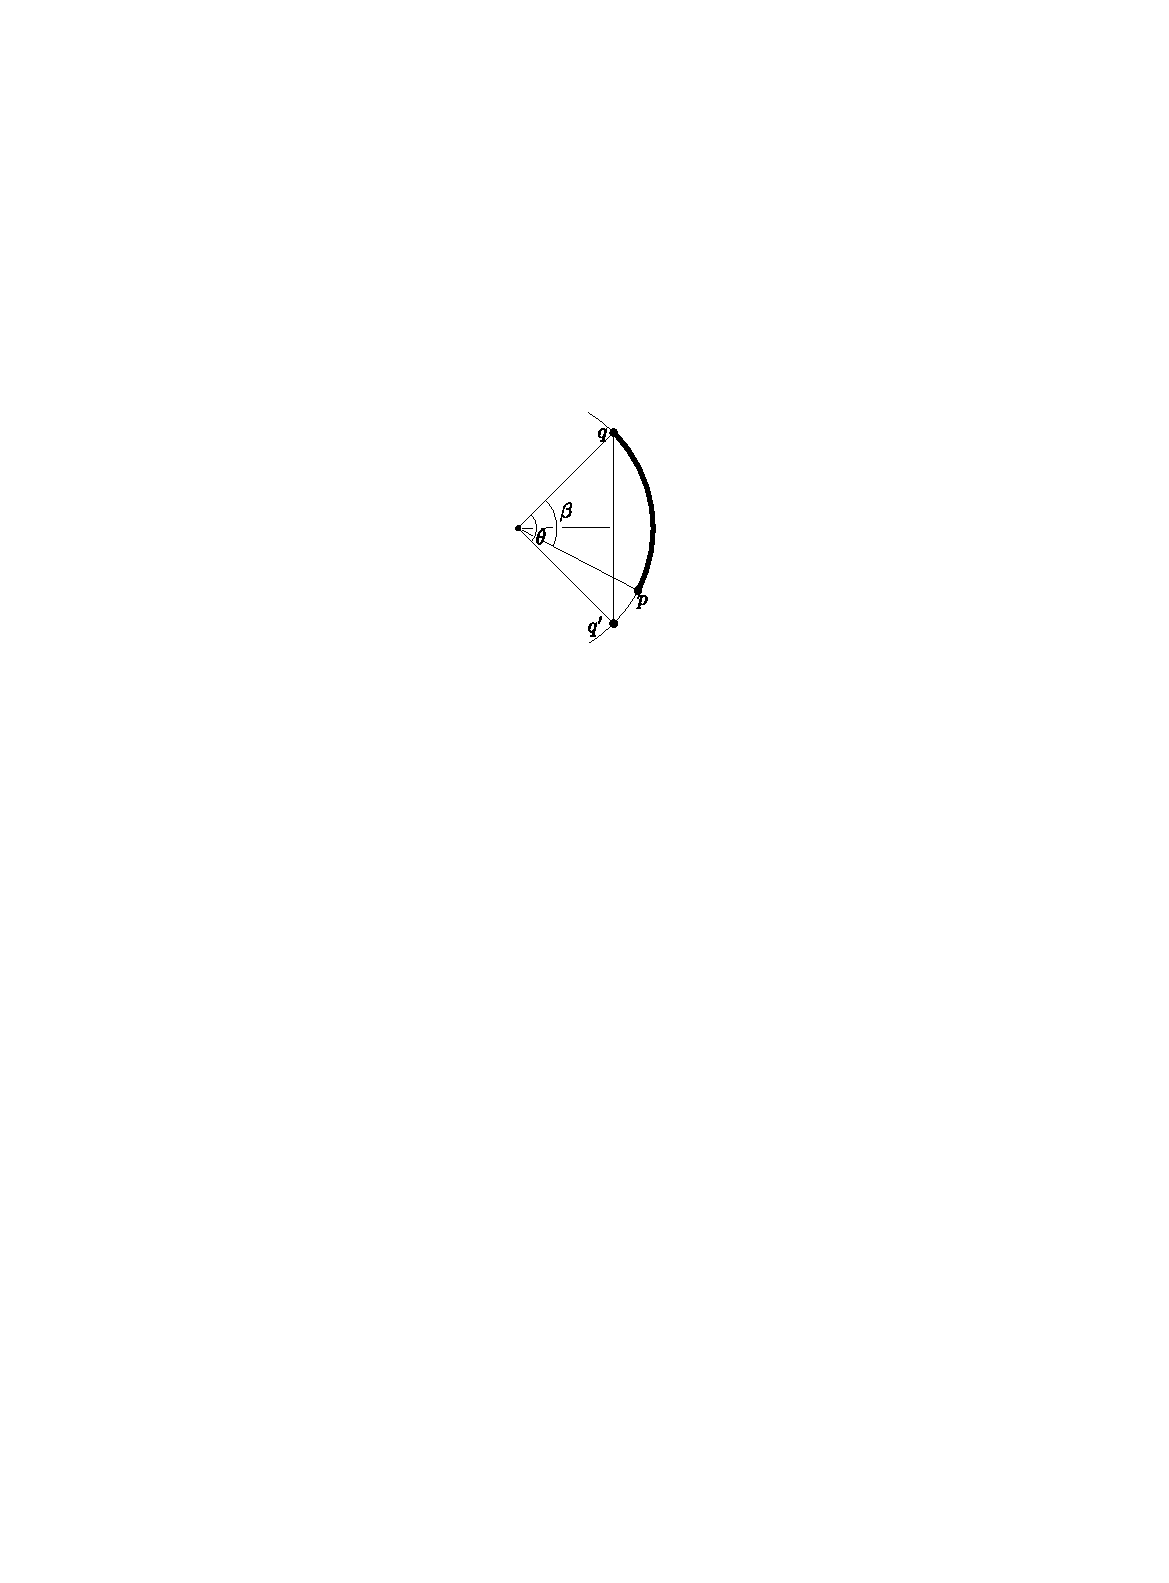
\includegraphics[width=.8\textwidth]{Figures/Bose_a.pdf}
            \caption[]%
            {{}}    
            \label{fig:Bose_a}
        \end{subfigure}
        \hfill
        \begin{subfigure}[b]{0.475\textwidth}  
            \centering 
            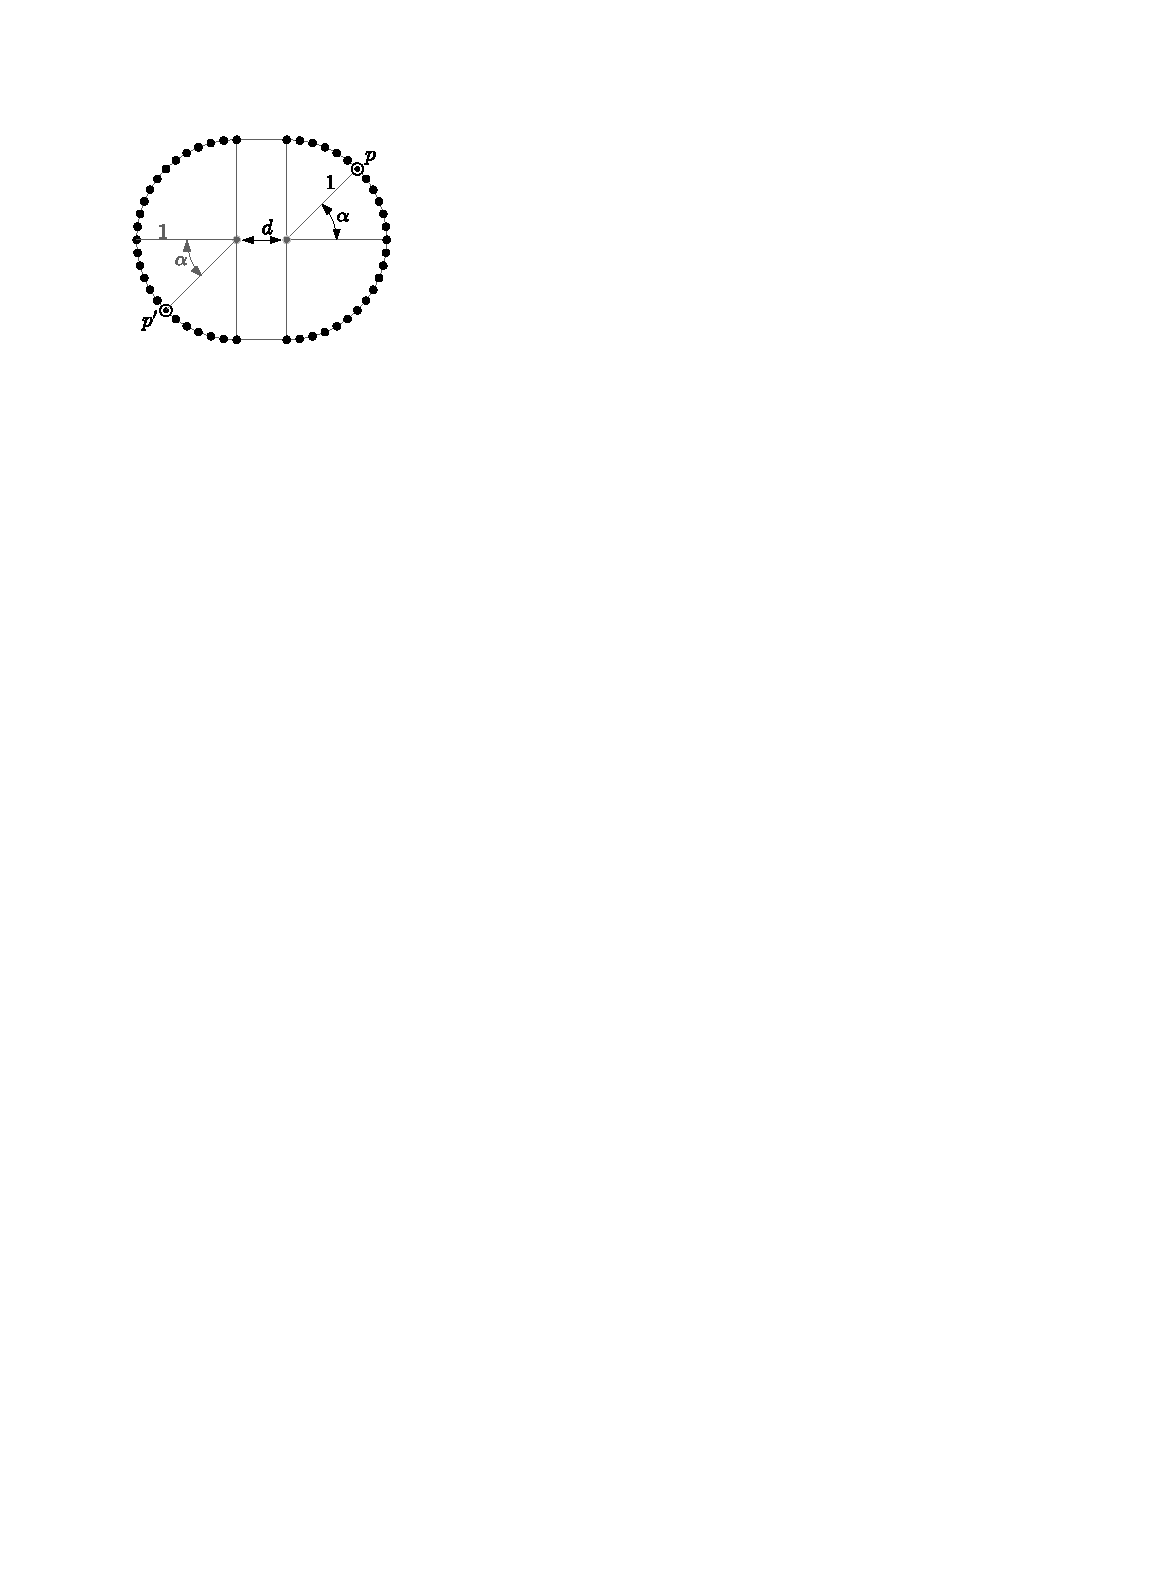
\includegraphics[width=.8\textwidth]{Figures/Bose_b.pdf}
            \caption[]%
            {{}}    
            \label{fig:Bose_b}
        \end{subfigure}
        \vskip\baselineskip
        \begin{subfigure}[b]{0.475\textwidth}   
            \centering 
            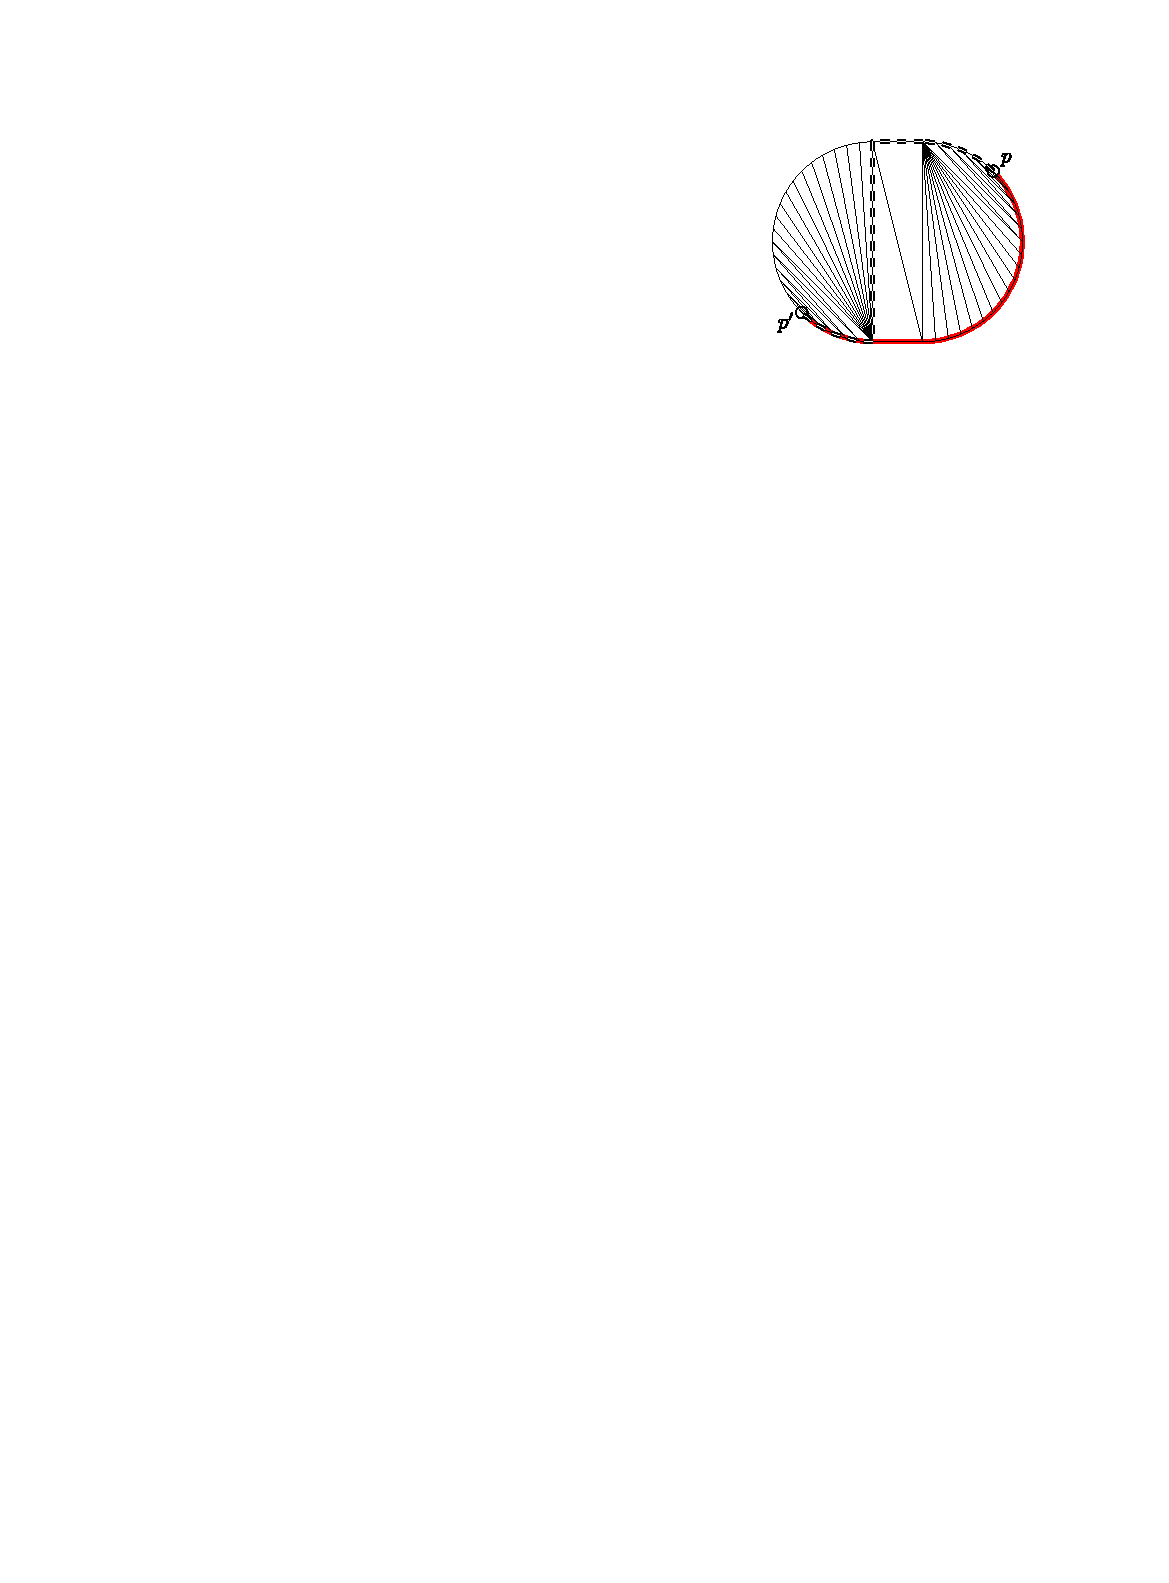
\includegraphics[width=.8\textwidth]{Figures/Bose_c.pdf}
            \caption[]%
            {{}}    
            \label{fig:Bose_c}
        \end{subfigure}
        \quad
        \begin{subfigure}[b]{0.475\textwidth}   
            \centering 
            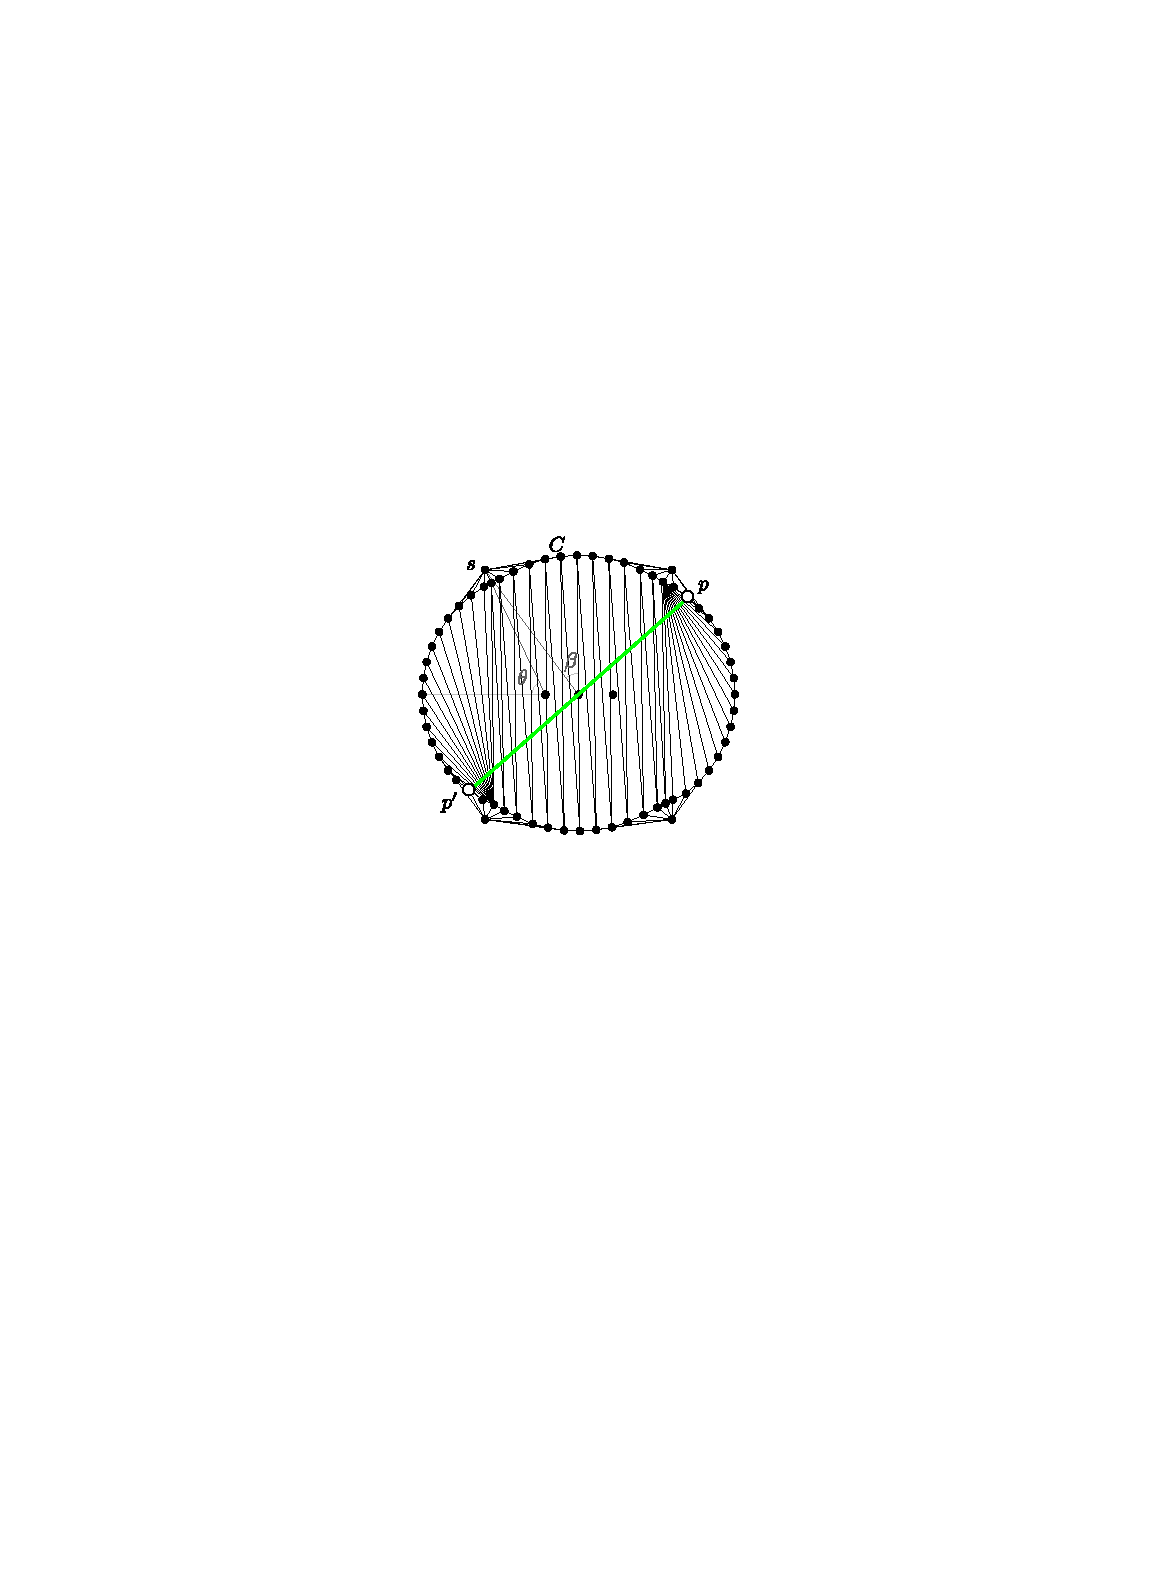
\includegraphics[width=.8\textwidth]{Figures/Bose_d.pdf}
            \caption[]%
            {}    
            \label{fig:Bose_d}
        \end{subfigure}
        \caption[Illustrations for the model proving a lower bound 1.5846]{Illustrations for the model proving a lower bound 1.5846. \ref{fig:Bose_a} illustrates two types of locally optimal paths from $p$ to $q$.  \ref{fig:Bose_b} and  \ref{fig:Bose_c} give the construction for point set in convex position, a more general case comparing with the topic we study.  \ref{fig:Bose_d} is the instance with a stretch factor of 1.5846. Reprinted from \cite{BoseCGTA}.} 
        \label{fig:Bose}
    \end{figure}





\subsection{\texorpdfstring{$1.5932$}{Lg}, Xia and Zhang in 2011}
Xia and Zhang\cite{fwcg2010} improved the lower bound to  $1.5932$ in  2011 by reducing the problem to studying the stretch factor of a family of chains satisfying certain structural properties. According to  \cite{dobkin}, we know that the maximum stretch factor among all chains made by $n+1$ circles is always greater than the maximum stretch factor among claims with  $n$ circles. Thus, they aimed to establish a well-defined family of chains such that every chain has the maximum stretch factor among all chains made by the same number of circles.
Figure~\ref{fig:ZX} gives an illustration of the chains with worse bounds.




\begin{figure}[ht]
\hspace*{\fill}
\begin{subfigure}{0.45\textwidth}
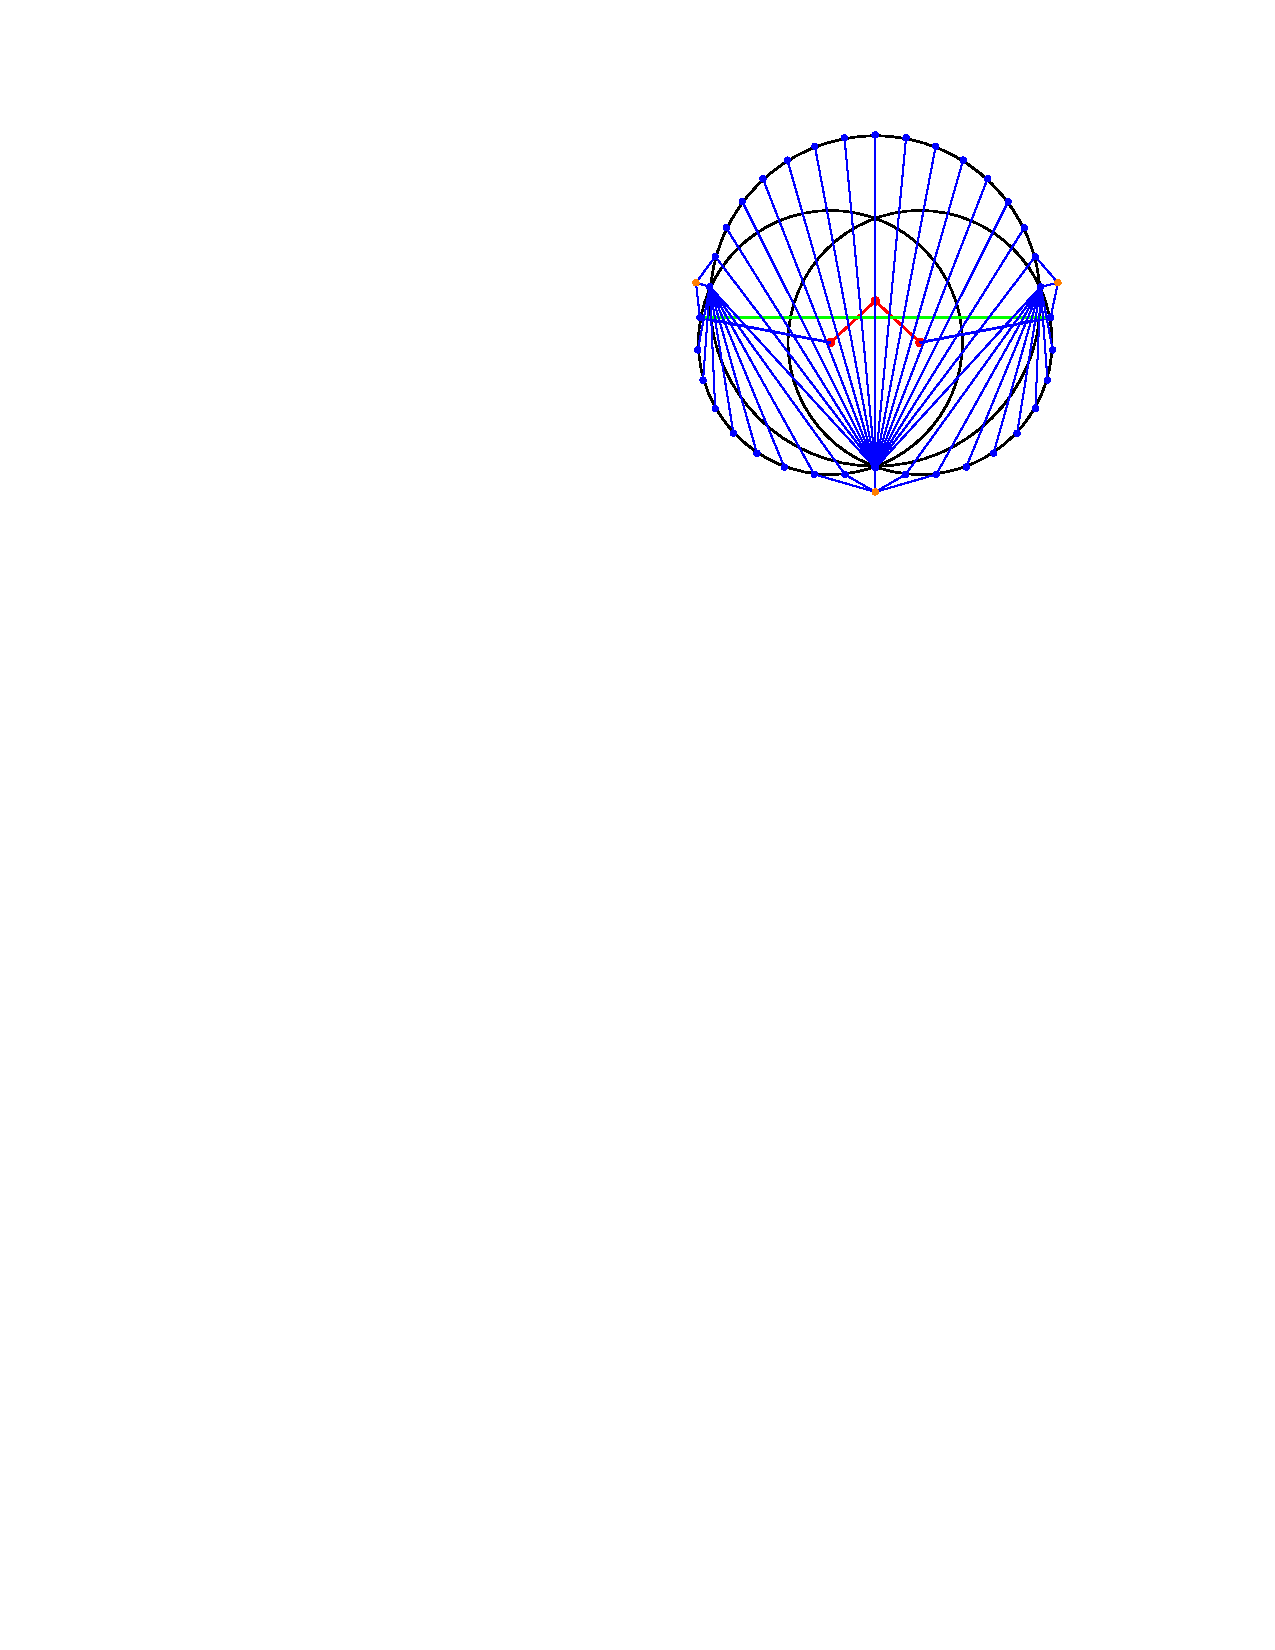
\includegraphics[width=\linewidth]{Figures/ZX_3.pdf}
\caption{} \label{fig:ZX_3}
\end{subfigure}
\hspace*{\fill} % separation between the subfigures
\begin{subfigure}{0.45\textwidth}
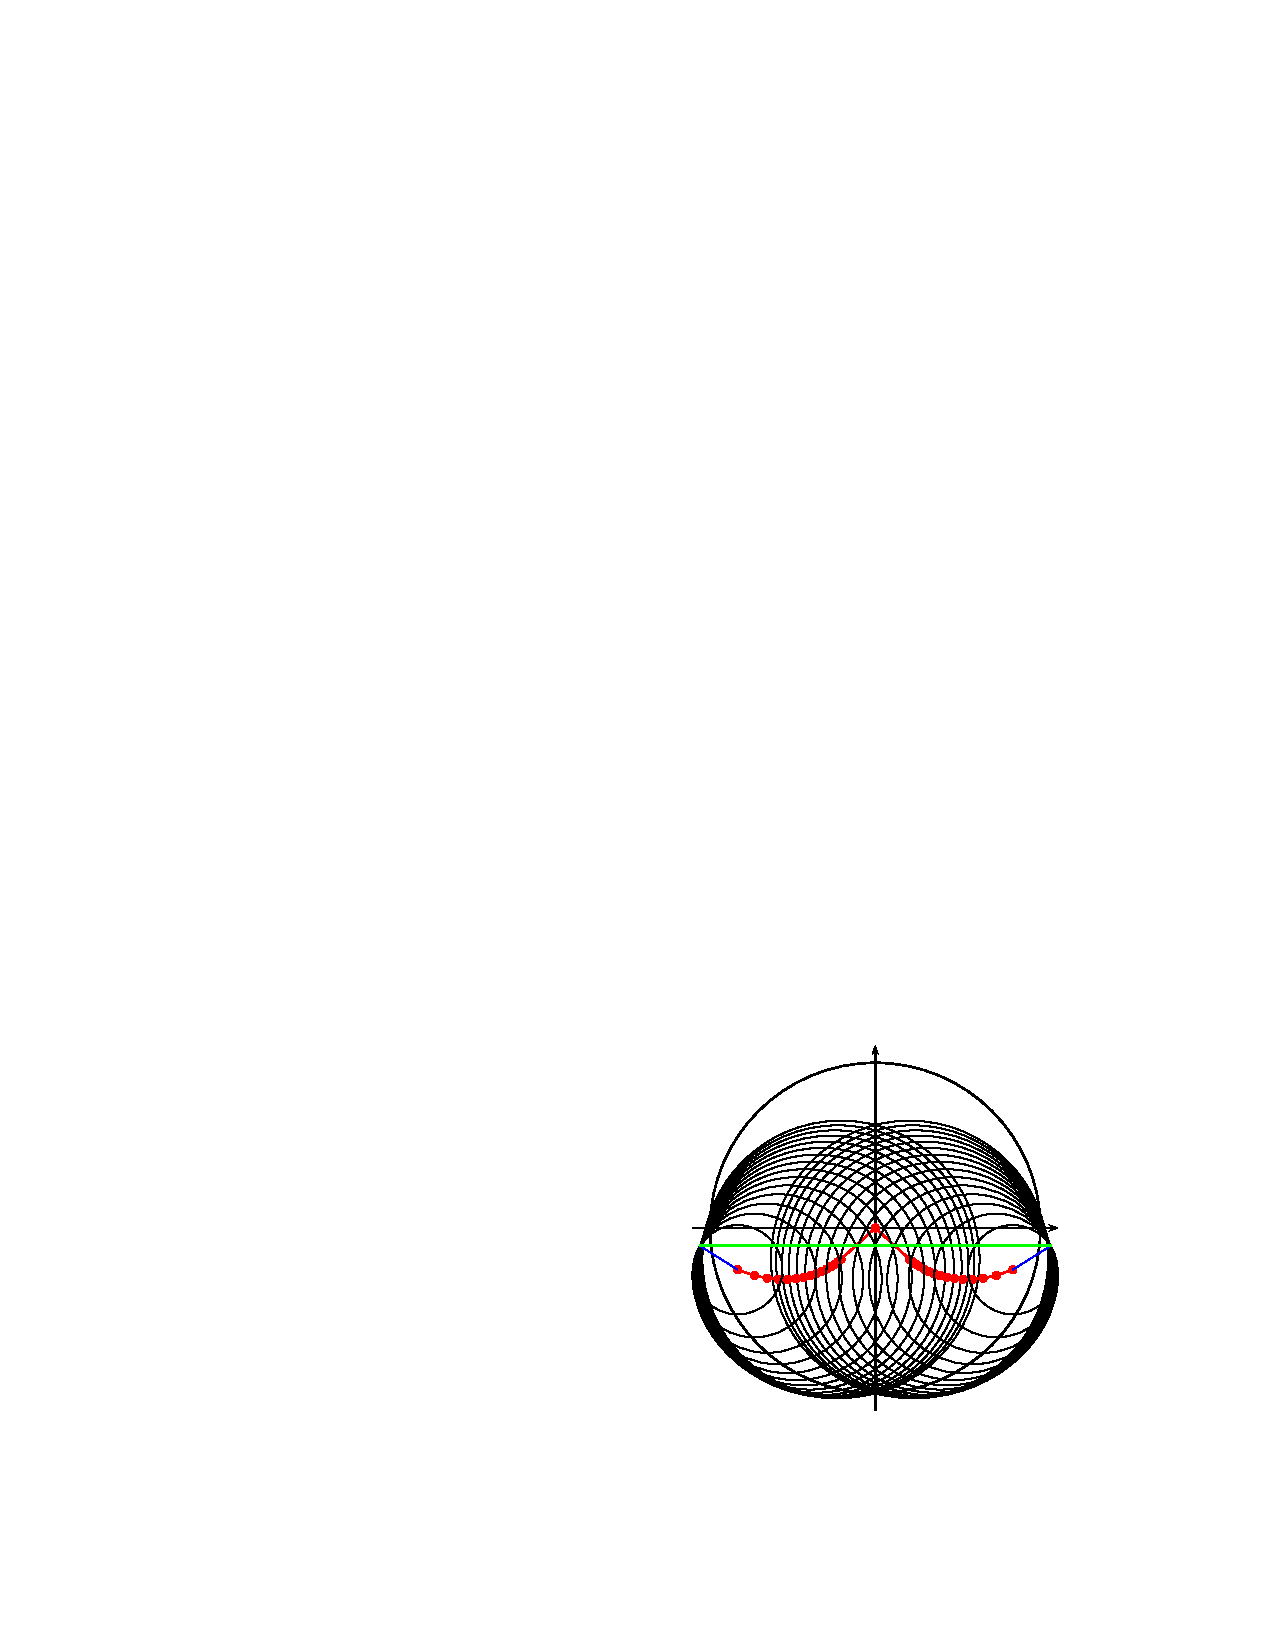
\includegraphics[width=\linewidth]{Figures/ZX_31.pdf}
\caption{} \label{fig:ZX_31}
\end{subfigure}
\hspace*{\fill}
\caption[A chain of circles with the stretch factor $1.5932$]{An instance for stretch factor $1.5932$. \ref{fig:ZX_3} shows shield points and edges in the basic case, a chain of three circles. \ref{fig:ZX_31} is a chain of circles with stretch factor $1.5932$. Reprinted from \cite{fwcg2010}.} \label{fig:ZX}
\end{figure}








\subsection{\texorpdfstring{$1.59324$}{Lg}, Snoeyink and Verma in 2012}
Snoeyink and Verma used a  characterization to bring both upper and lower bounds closer to 1.6 in \cite{arcgon}. Instead of converting a point set into a chain of circles, they transformed the original model to a class of graphs called arcgon. Basically, an arcgon is an embedded graph made up by three types of faces shown  Figure~\ref{fig:SV}. An arcgon is similar with a chain of circles in \cite{fwcg2010}, but this definition makes them characterize edges more convenient. They conjectured that if a arcgon has the greatest stretch factor among all arcgons with the same faces, every path should be the shortest path. That is, every path has the same length. For the lower bound part, they constructed a arcgon following their conjecture and stated its stretch factor  is $1.5846$. But they did not provided the exact parameters in this paper. 







\begin{figure}[ht]
\centering
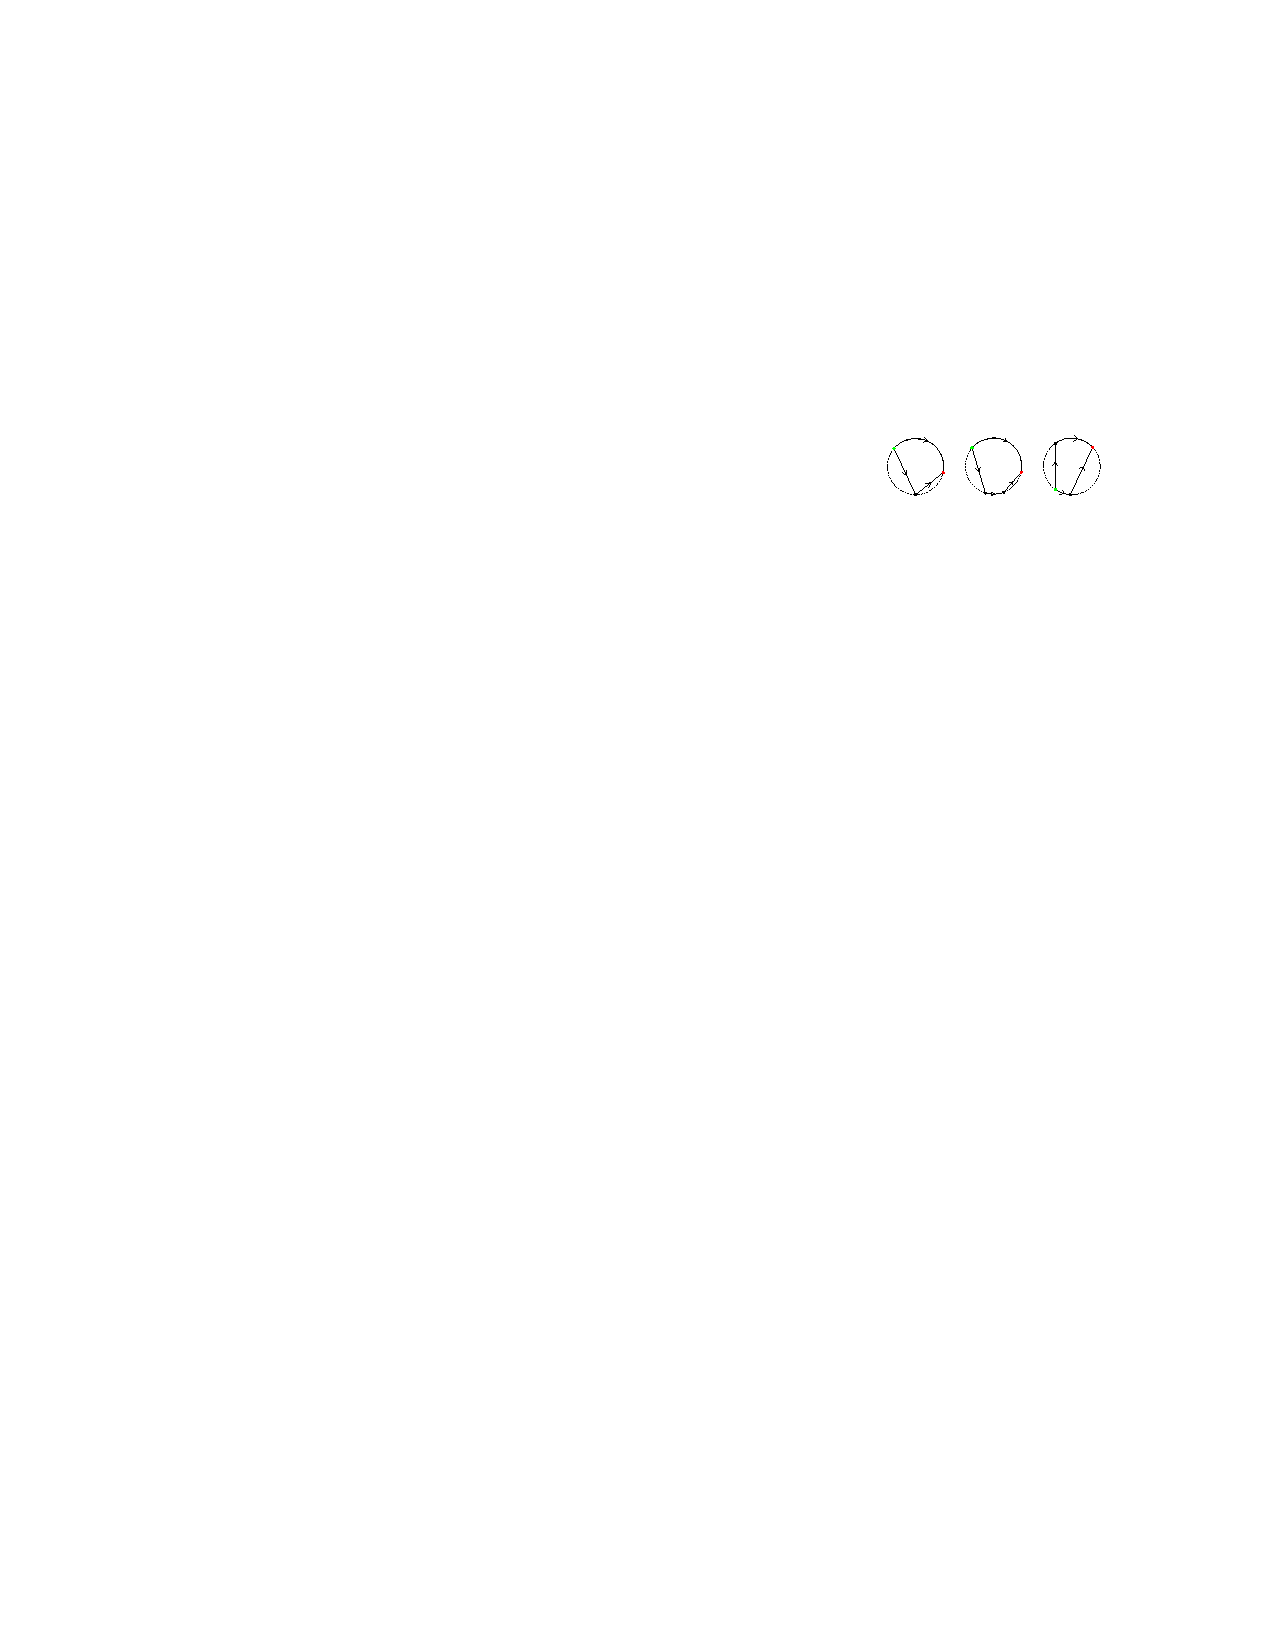
\includegraphics[width=100mm]{Figures/SV.pdf}
% \decoRule
\caption[Tree types of faces in arcgons]{Tree types of faces in arcgons. Reprinted from \cite{xia}.} 
\label{fig:SV}
\end{figure}






\section{On the Upper Bound}

\subsection{\texorpdfstring{$5.08$}{Lg},  Dobkin, Friedman, and Supowit in 1987}
The upper bound for the stretch factor was first shown by Dobkin, Friedman, and Supowit. They proved that all stretch factor of the Delaunay triangulation is at most $5.08$.  illustrates two types of paths from one end point on the $x$-axis $a$ to the other end point $b$. The path in Figure~\ref{fig:DFS_a} is called one-sided because all its intermediate points $b's$ are on one side of the $x$-axis. Then, since the length of the one-sided path from $a$ to $b$ could not be longer than the perimeter of the semicircle with a diameter $ab$, its stretch factor is at most $\pi/2$. 

We may also meet a case that the path is not even close to being ones-sided. For example, the path in Figure~\ref{fig:DFS_b} goes below the $x$-axis after $b_1$ and comes back to the positive range after $b_4$. For all such cases, Dobkin, Friedman and Supowit showed that the path length is at most $(1+\sqrt{5})$ times of the horizontal distance. Therefore, summing over all those sub-paths  would give a total path length at most $((1+\sqrt{5})/2)\pi$ times of  the distance. Therefore, they concluded the stretch factor of the Delaunay triangulation is at most $((1+\sqrt{5})/2)\pi\approx 5.08
$.




\begin{figure}[ht]
\begin{subfigure}{0.48\textwidth}
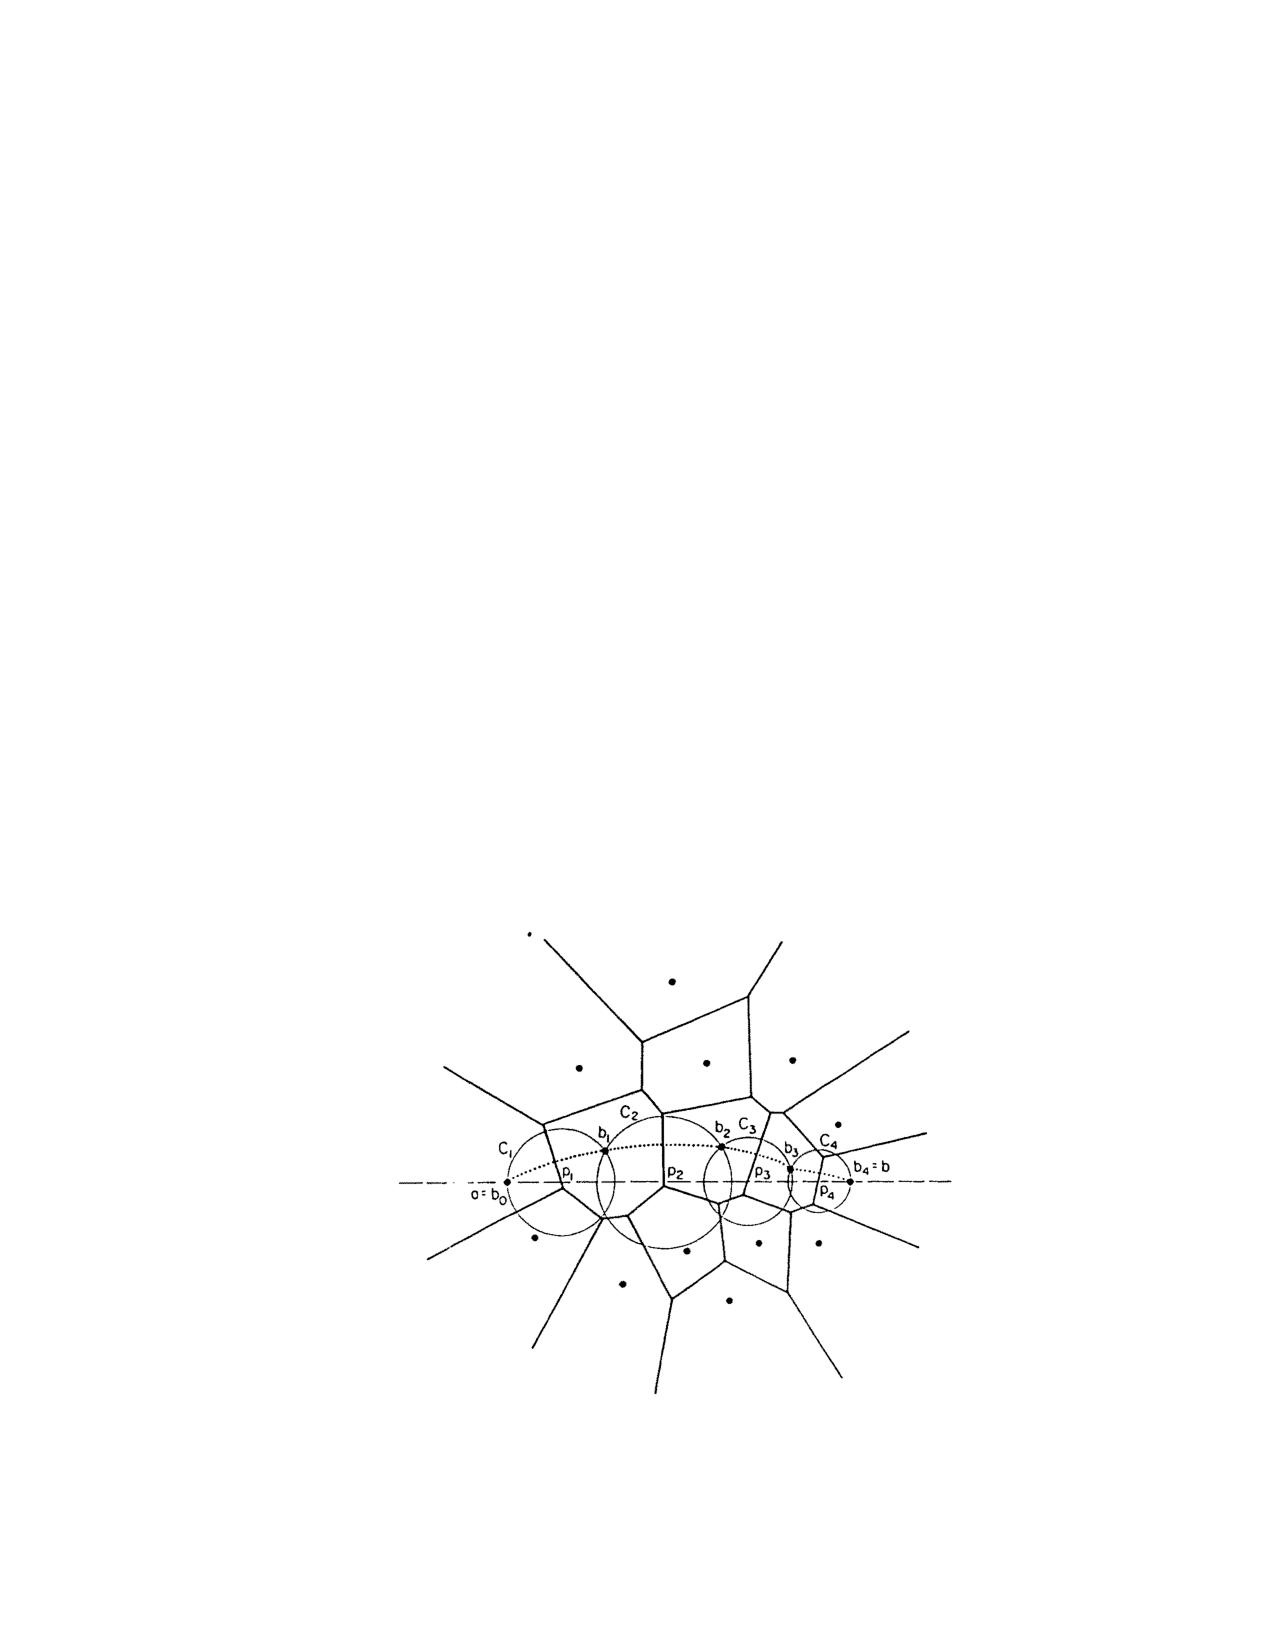
\includegraphics[width=\linewidth]{Figures/DFS_a.pdf}
\caption{} \label{fig:DFS_a}
\end{subfigure}
\hspace*{\fill}
\begin{subfigure}{0.48\textwidth}
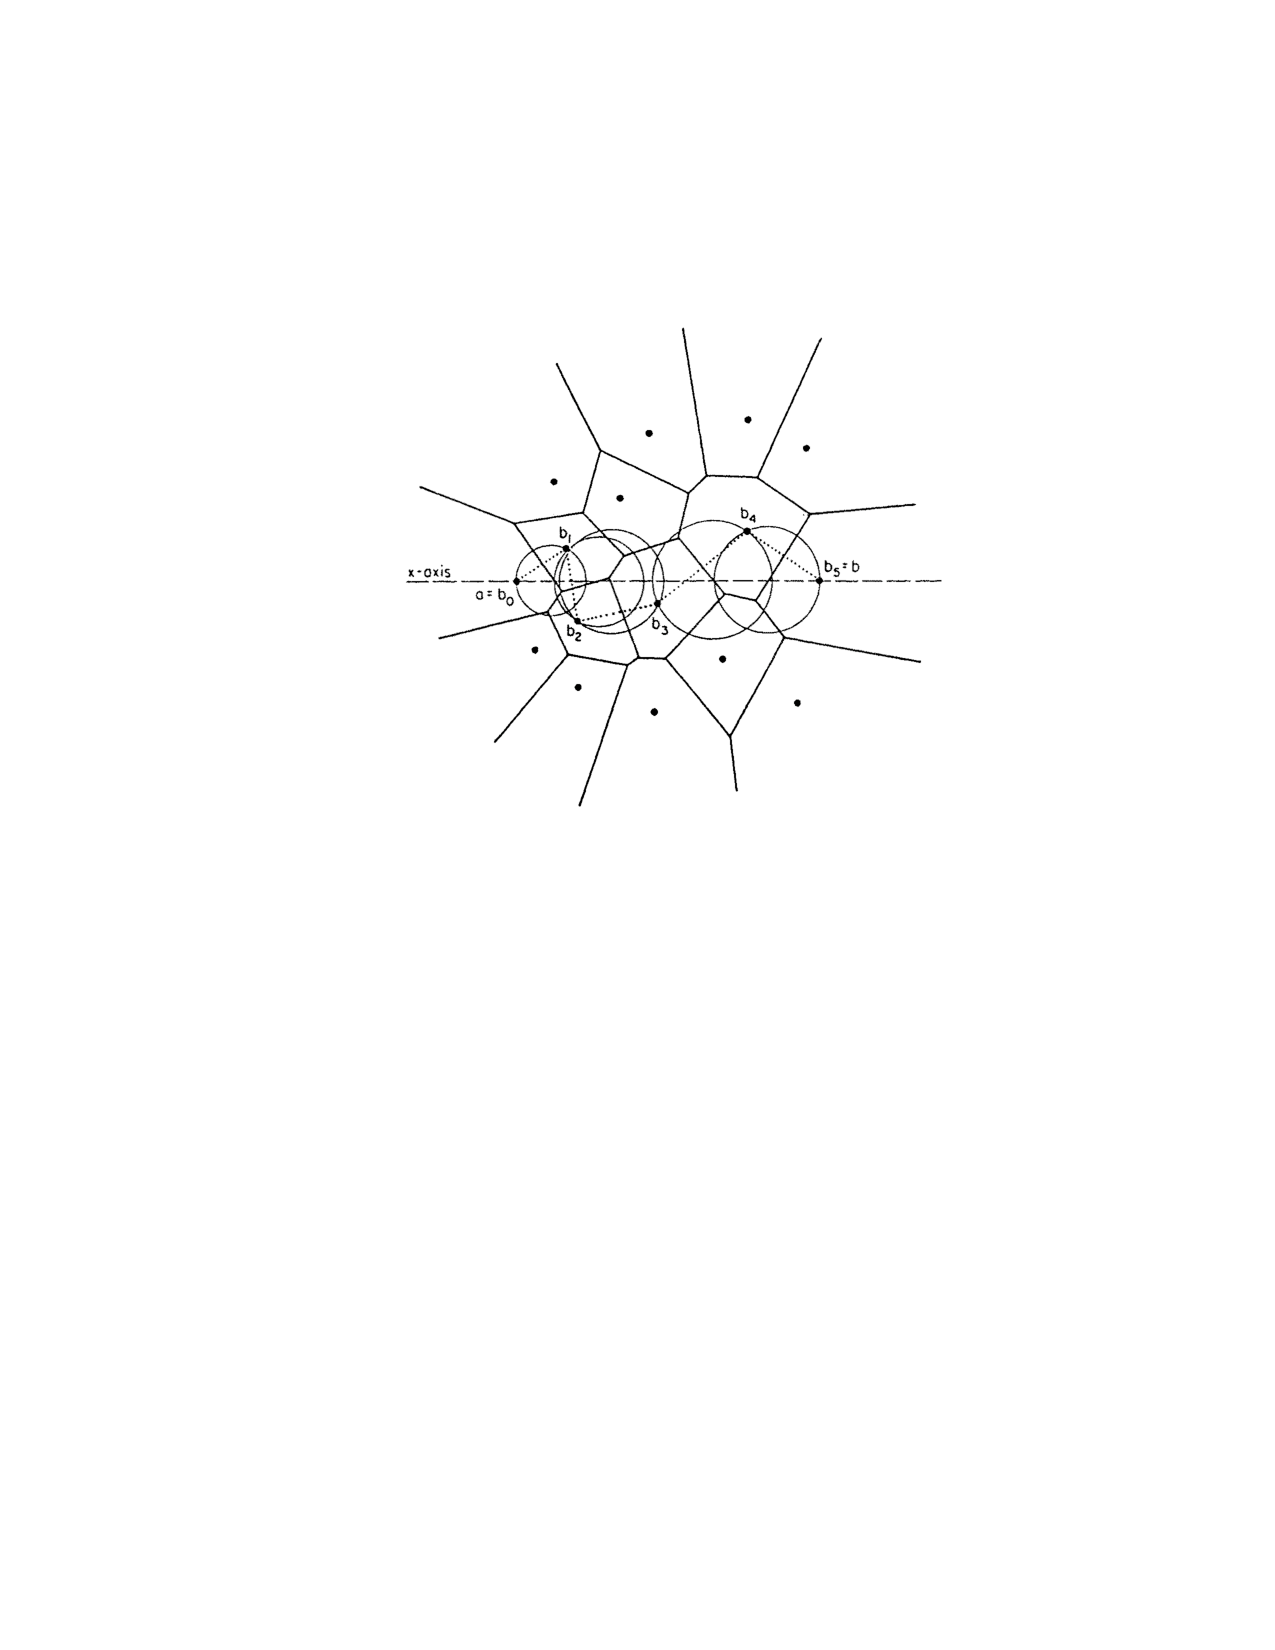
\includegraphics[width=\linewidth]{Figures/DFS_b.pdf}
\caption{} \label{fig:DFS_b}
\end{subfigure}
\hspace*{\fill} % separation between the subfigures
\caption[A one-sided path and a non one-sided path]{One-sided path and non one-sided path. Reprinted from \cite{dobkin}.} \label{fig:DFS}
\end{figure}


\subsection{\texorpdfstring{$2.42$}{Lg},  Keil and Gutwin in 1989}  
In 1989,  Keil and Gutwin published a paper\cite{keil} to discuss two classes of graphs which approximate the complete graph. One is the graph of the Delaunay triangulation. By analyzing they proved an upper bound of $2.42$. 

\subsection{\texorpdfstring{$1.998$}{Lg},  Xia in 2011}  
An upper bound of $1.998$ was shown by Xia\cite{xia} in 2011 with a different approach from the previous work. This approach in based on the geometry of a chain of disks in the plane. Then, by carefully defining the stretch factor of a chain in analogy to that of  the Delaunay triangulation, one could prove bound on the stretch of the Delaunay triangulation in the model of chains. After converting the Delaunay triangulation problem to a chain of disks, Xia proceeded the inductive proof by amortized analysis.  



\subsection{\texorpdfstring{$1.636245$}{Lg} (Conjectured), Snoeyink and Verma in 2012}
As we mentioned in section 2.1.4, Snoeyink and Verma stated a conjecture that  a arcgon which has the greatest stretch factor among arcgons with the same faces must have equal length paths. They proved that the upper bound could be improved to $1.636245$ once the conjecture is shown.